\documentclass[a4paper,8pt]{beamer}
\mode<presentation>
{
  \usetheme{Boadilla}
  % possiblities Singapore, Malmoe, Dresden 
  \setbeamercovered{transparent}
}

 
%\setbeamertemplate{navigation symbols}{} 
% removes the navigation symbols

%color setting more or less matching U of A colors
\setbeamercolor*{palette secondary}{use=structure,fg=white,bg=structure.fg!55!black}
\setbeamercolor*{palette tertiary}{use=structure,fg=white,bg=red!50!black}
%\usetheme{Madrid}
%\usecolortheme{seahorse}
\usepackage[retainorgcmds]{IEEEtrantools}
\usepackage{graphicx}
\usepackage{physics}
\usepackage{bm,bbm}
\usepackage{tabularx,multirow,booktabs}
\usepackage{subcaption}
\usefonttheme{serif}
\title[Free energy]{Research update}
\date{\today}
\author{Sree Ganesh}
\institute[U of A]{Schwartz Group \\ University of Arizona}
\begin{document}
\maketitle
%
%------------------------------------------------------------------------------
% SLIDE 1
%------------------------------------------------------------------------------
%
%\begin{frame}
%\frametitle{Contents}
%\begin{itemize}
%  \item Introduction
%	\item Convergence tests
%	\item Hartree-Fock and the case of Conjugated acenes
%	\item Sodium clusters and inclusion of temperature effects
 %  \item Non-orbital-optimized RPA based polarizabilities 
%\end{itemize}
%\end{frame}
%------------------------------------------------------------------------------
%
%------------------------------------------------------------------------------
% SLIDE 6
%------------------------------------------------------------------------------
%
\begin{frame}
\frametitle{Free energies from TPS}
\begin{figure}
\includegraphics[scale=0.5]{figures/free_energy.pdf}
\end{figure}
\end{frame}
\begin{frame}
%\frametitle{Free energies from TPS}
%\begin{figure}
%\includegraphics[scale=0.25]{hist_path/non_reac_path.pdf}
%\end{figure} 
%\pause
    \begin{figure}[ht]
        \begin{minipage}[b]{0.45\linewidth}
            \centering
            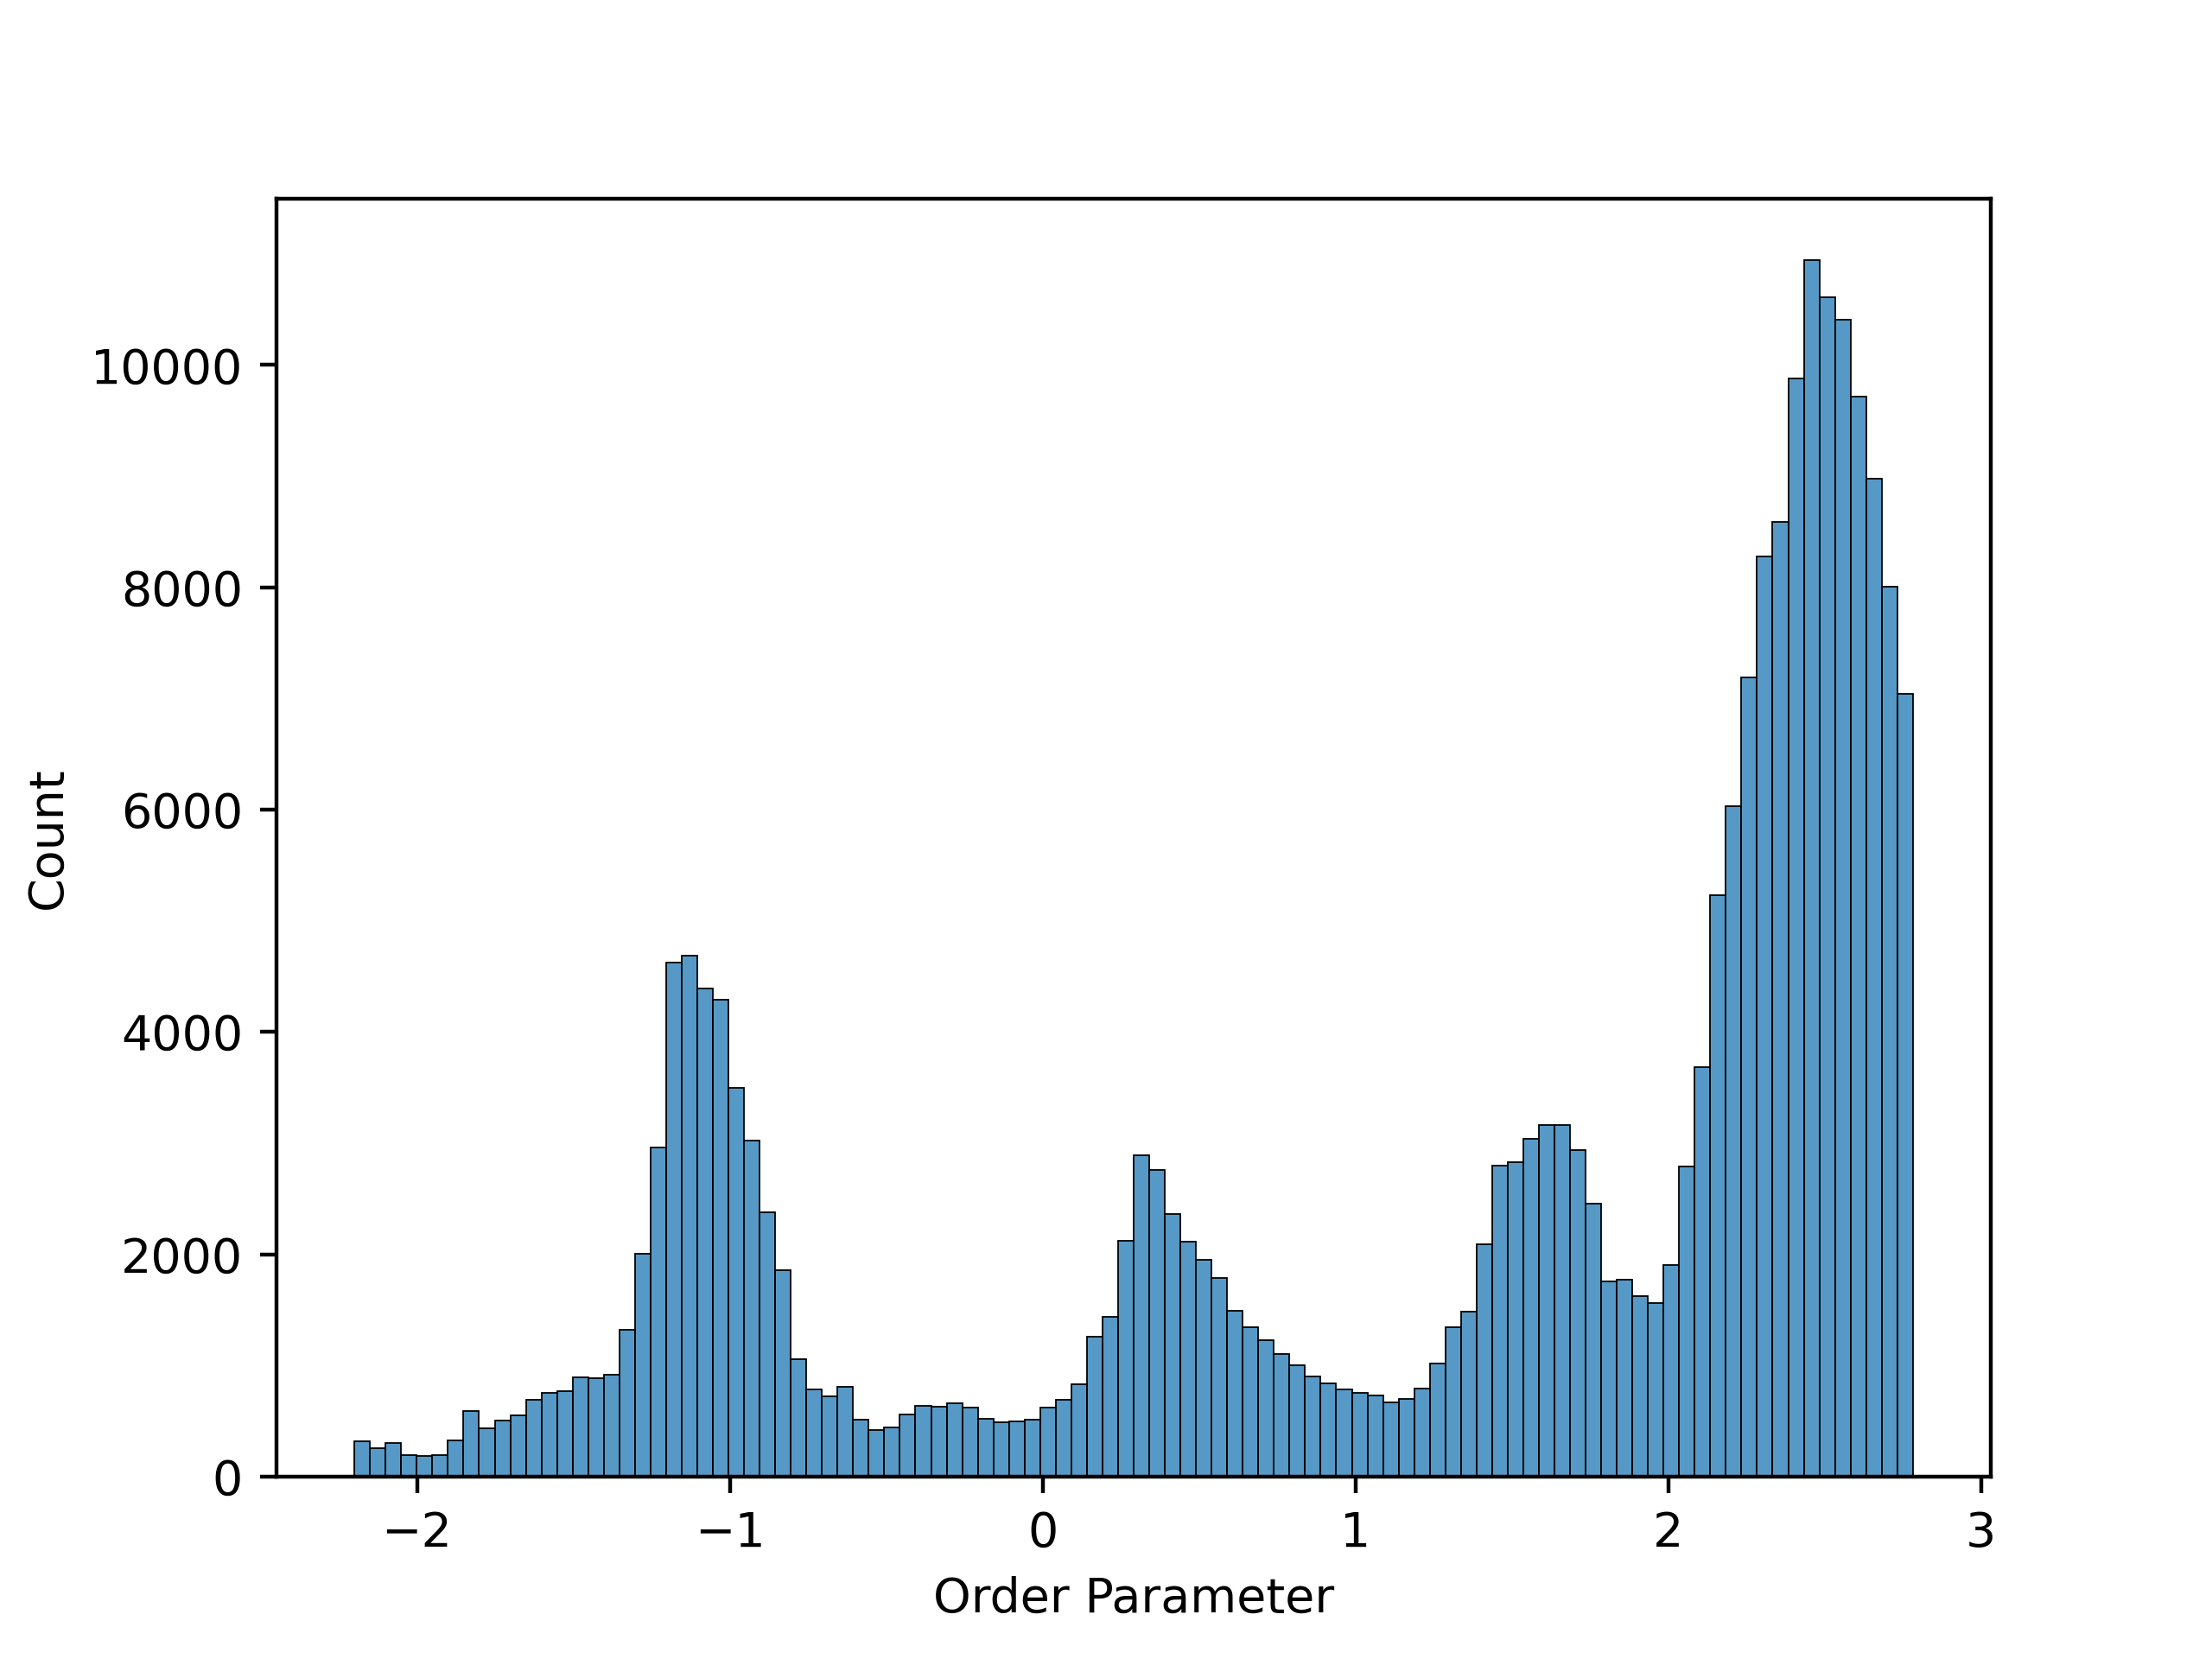
\includegraphics[width=\textwidth]{figures/1r_600n.png}
            \caption{Reac. traj. = 1, Non Reac. traj. =600}
            \label{fig:a}
        \end{minipage}
        \hspace{0.5cm}
        \begin{minipage}[b]{0.45\linewidth}
            \centering
            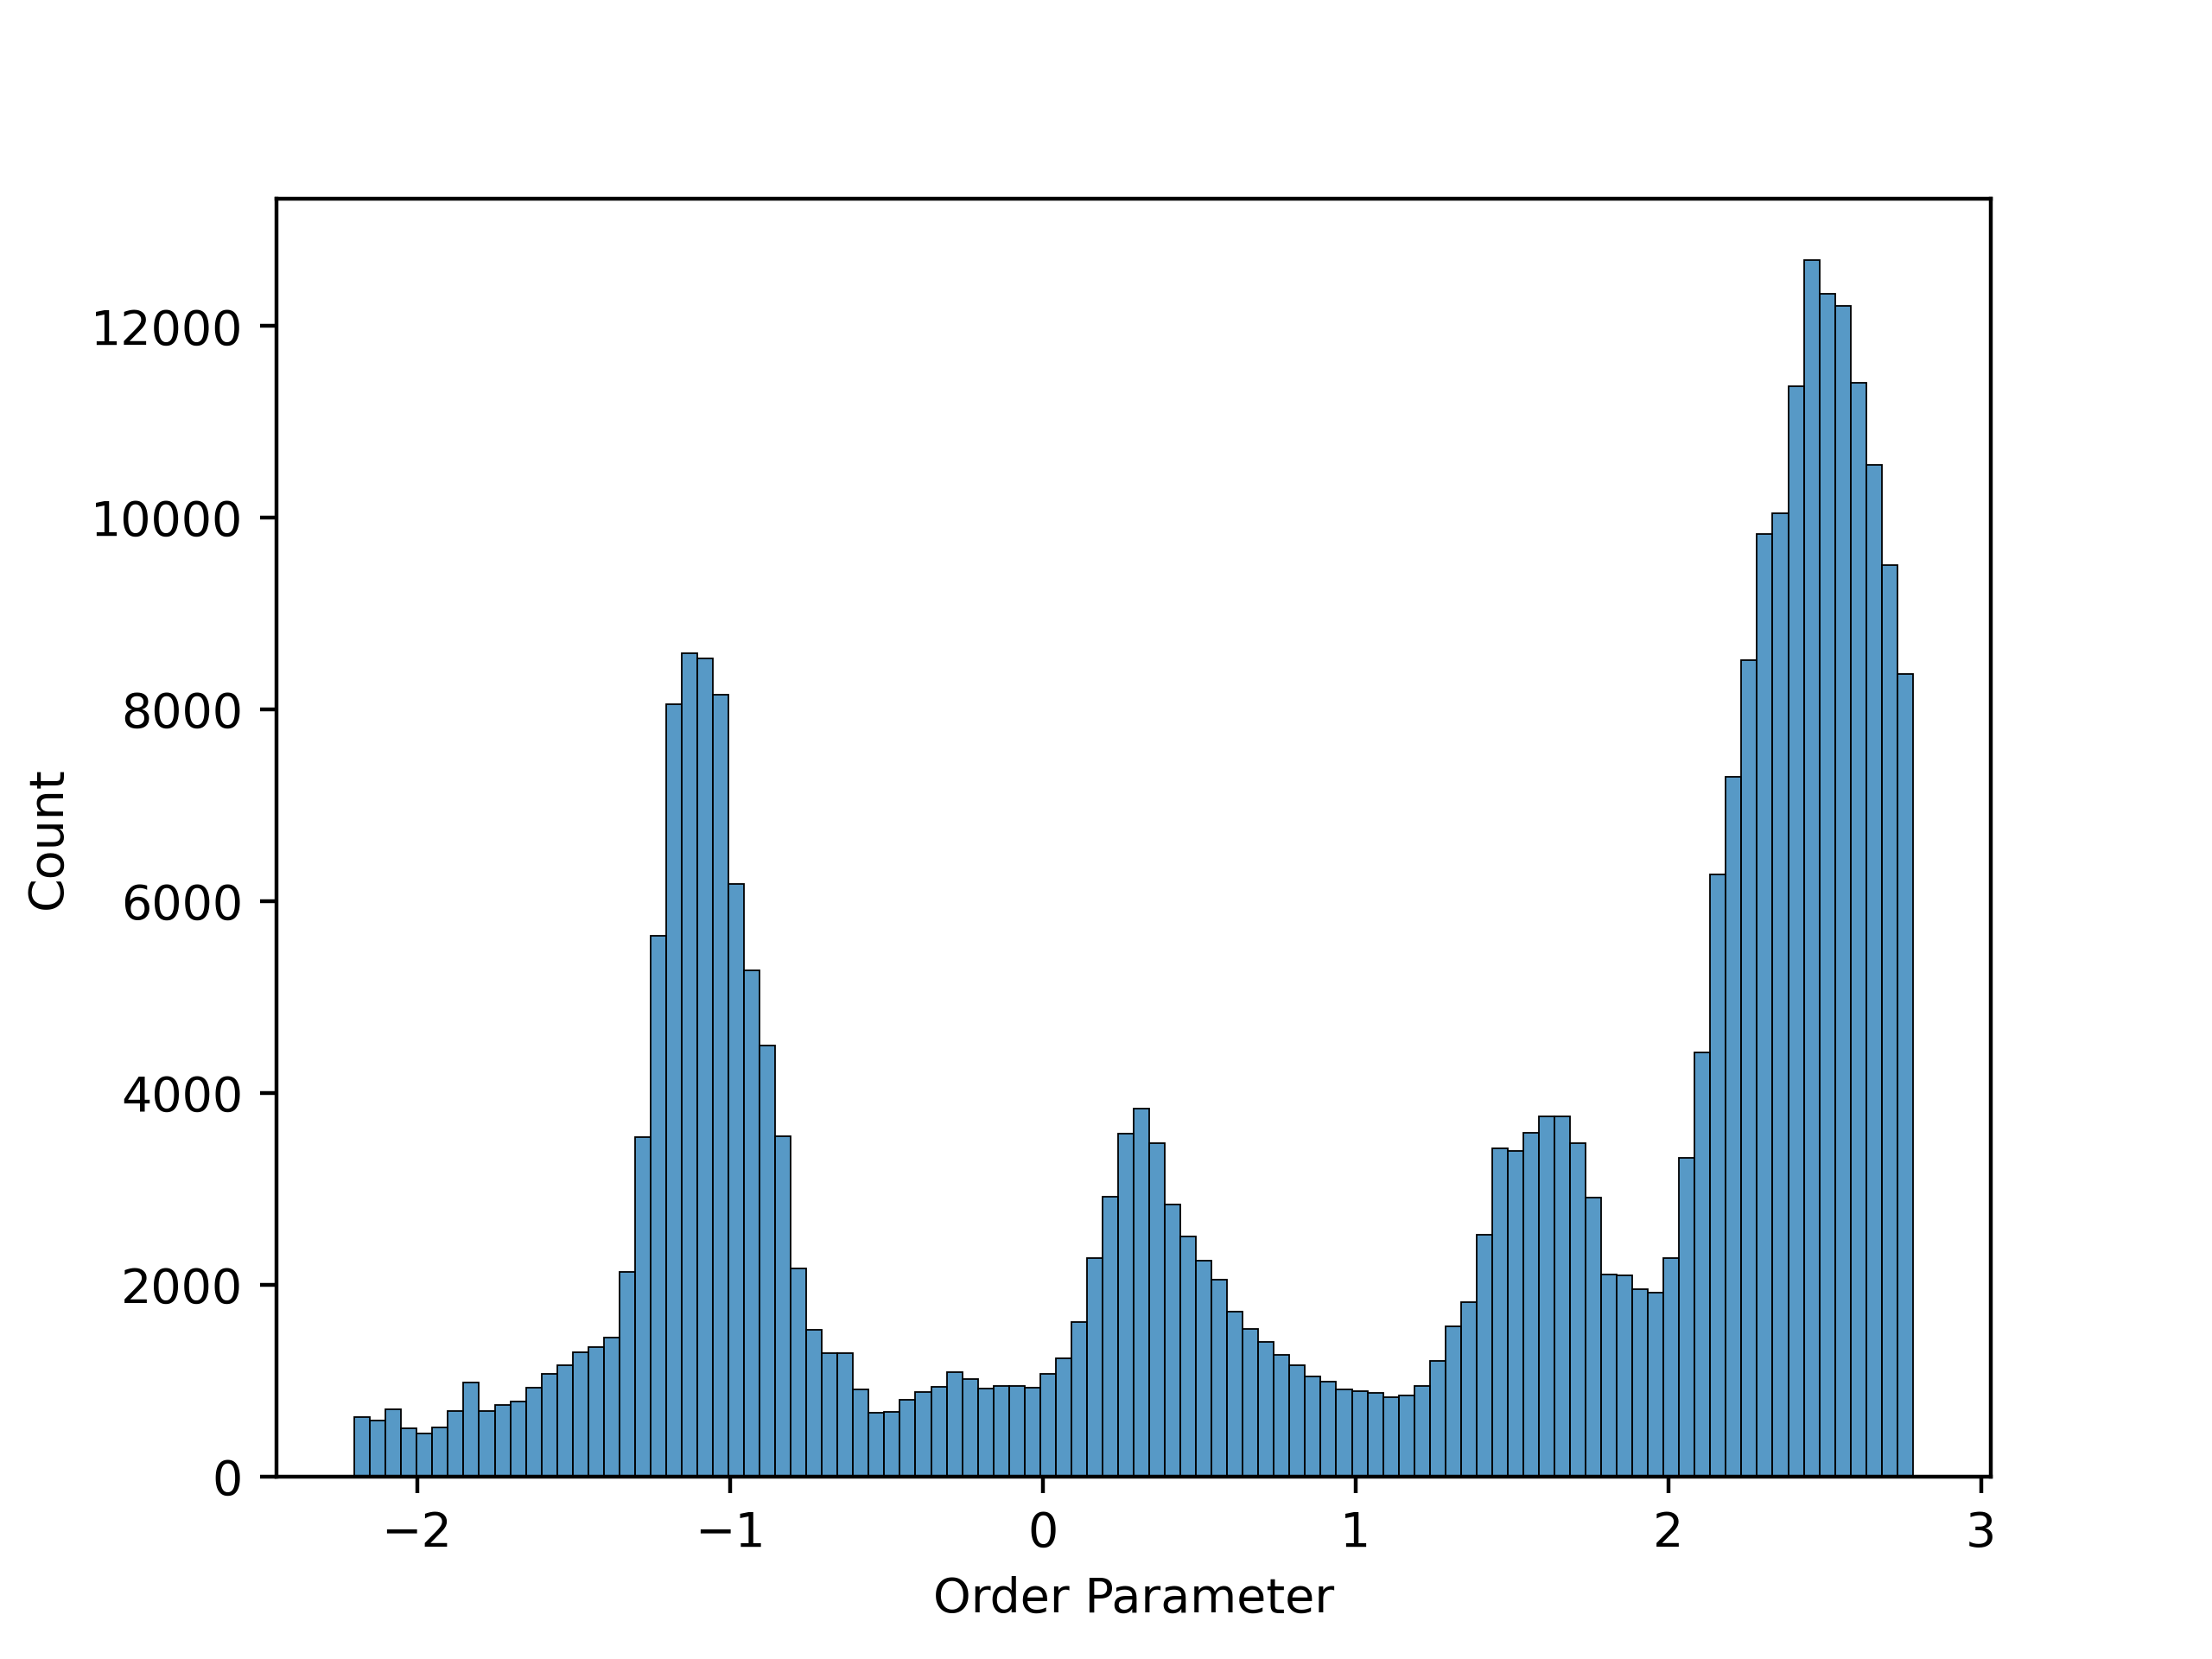
\includegraphics[width=\textwidth]{figures/190r_600n.png}
            \caption{Reac. traj. = 190, Non Reac. traj. =600}
            %\caption{QM region $+$ ARG 264, ARG 249, GLN 113 and SER 114 constrained.}
            \label{fig:b}
        \end{minipage}
    \end{figure}
\end{frame}
%
\begin{frame}
\frametitle{Committor distribution analysis of MAT2A enzyme catalysis}
%\begin{figure}
%\includegraphics[scale=0.25]{hist_path/non_reac_path.pdf}
%\end{figure} 
%\pause
    \begin{figure}[ht]
        \begin{minipage}[b]{0.45\linewidth}
            \centering
            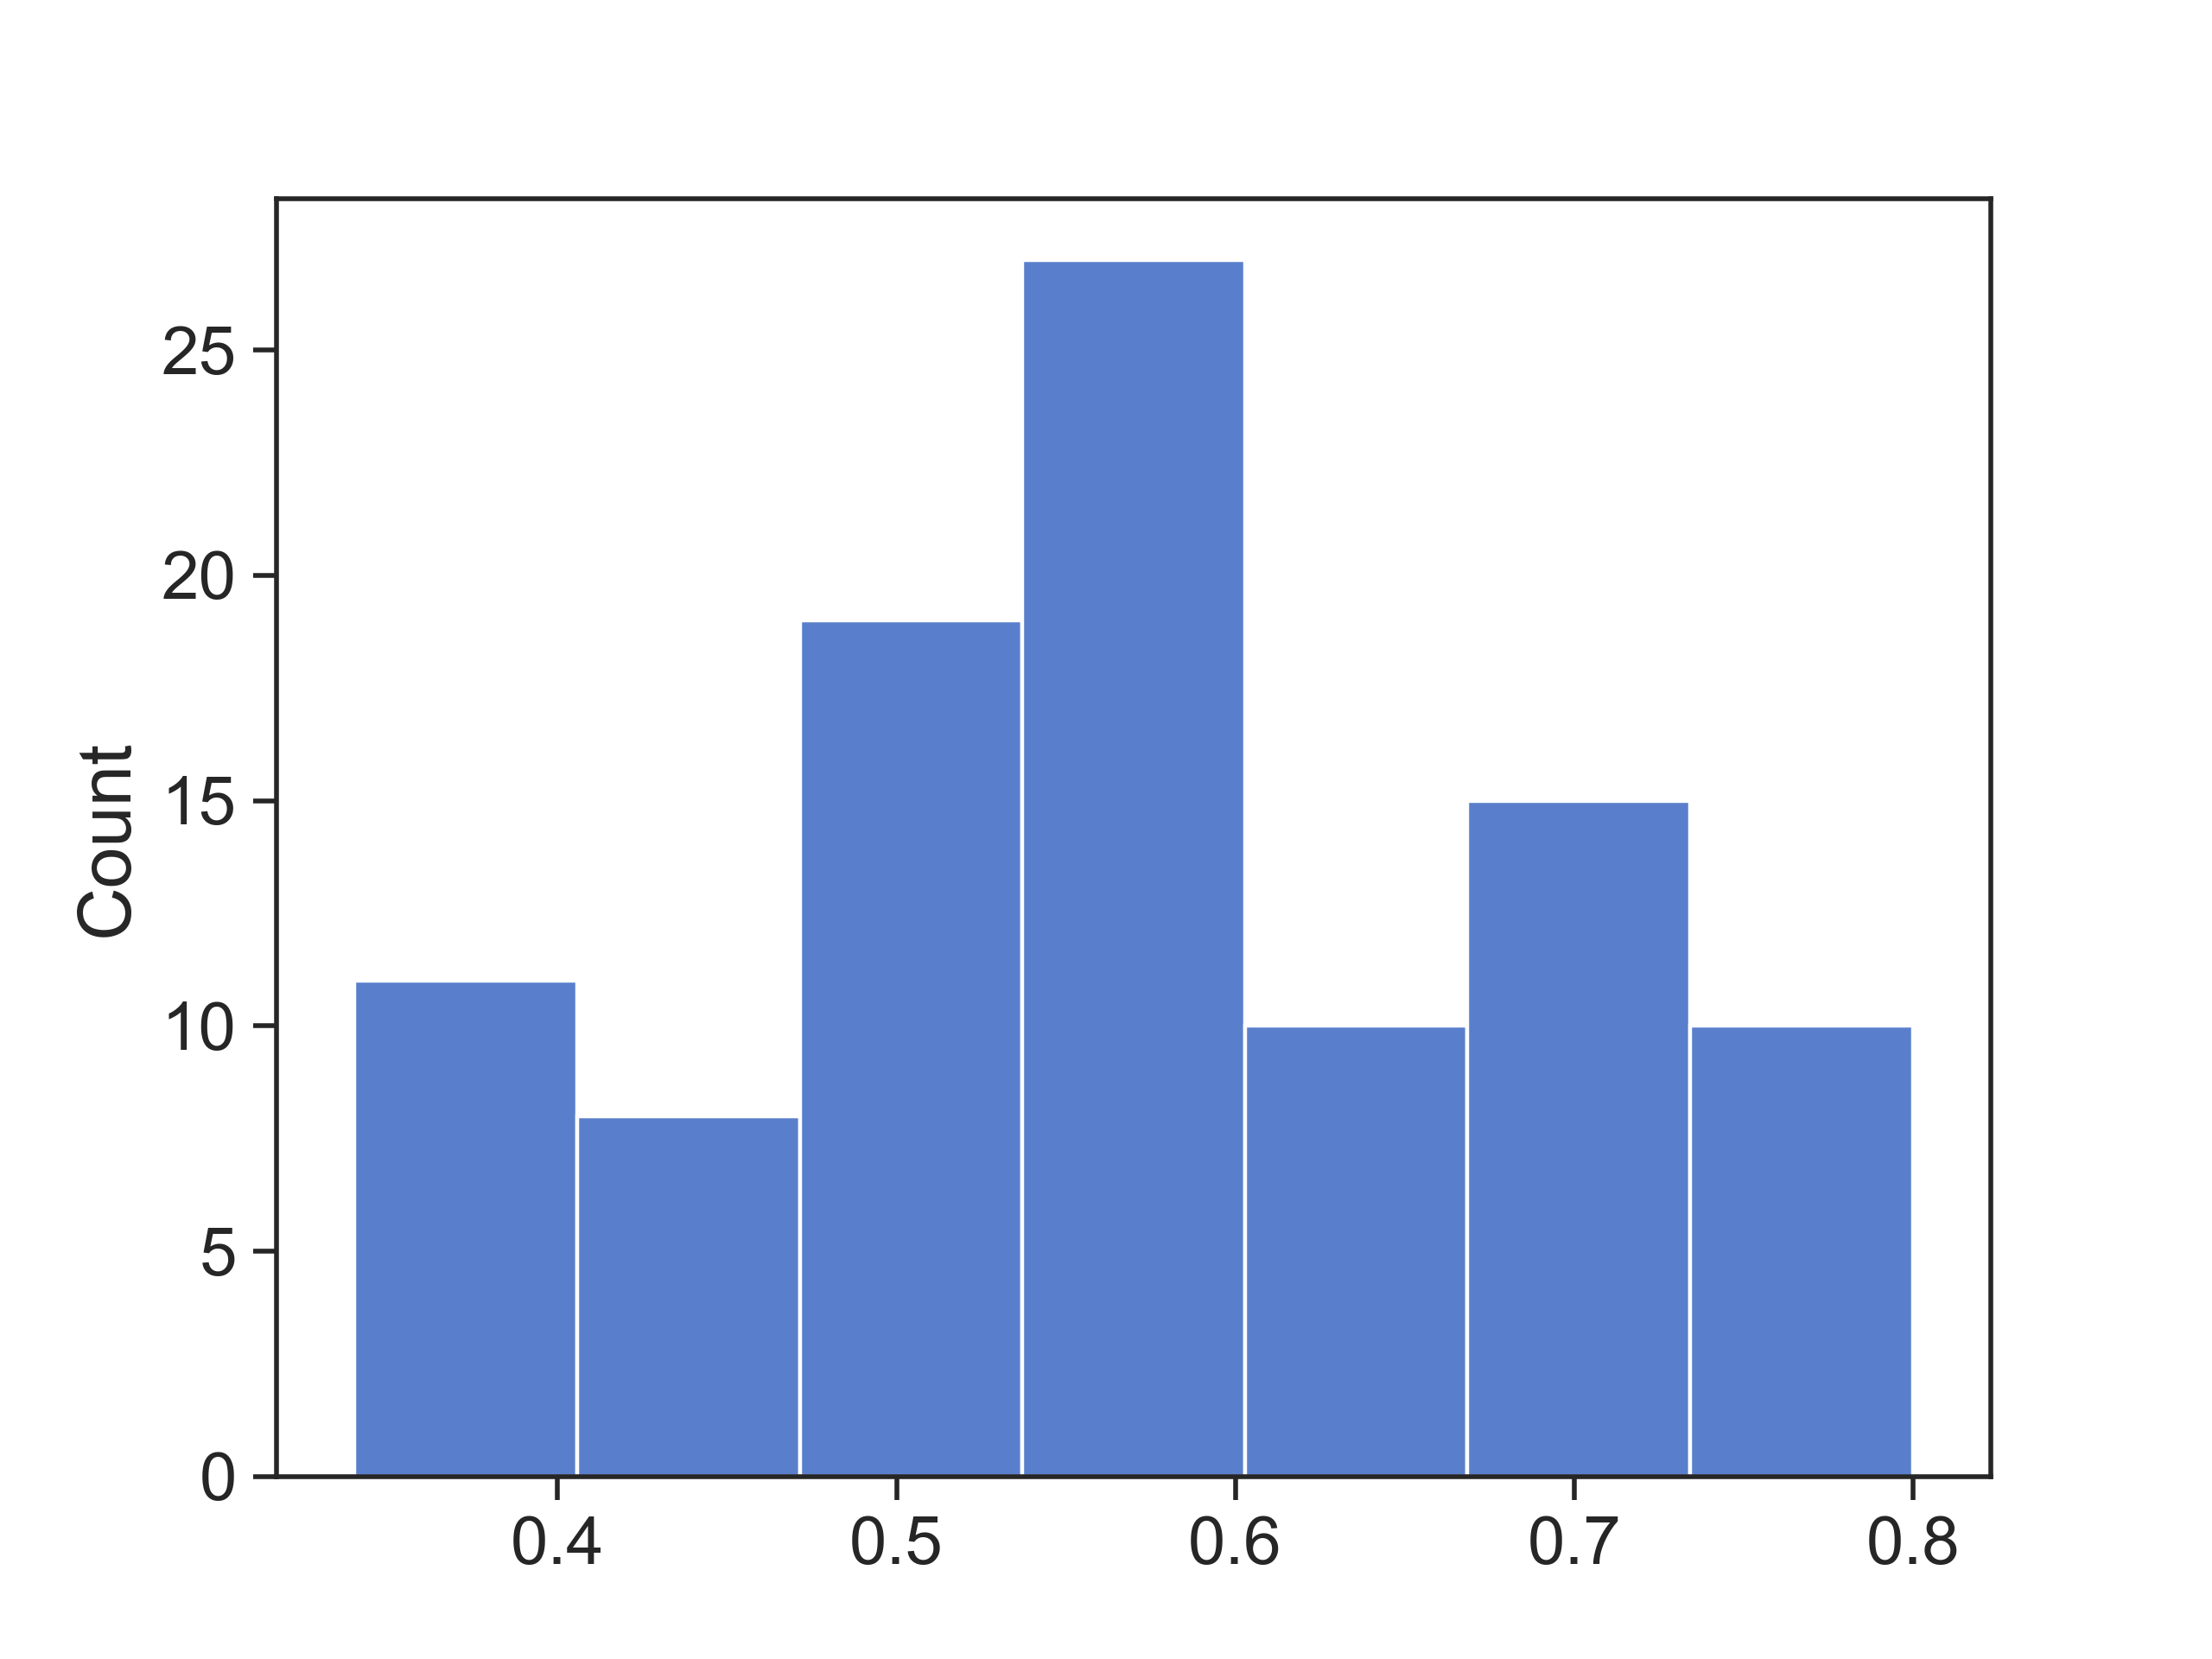
\includegraphics[width=\textwidth]{figures/40.png}
            \caption{QM region constrained.}
            \label{fig:a}
        \end{minipage}
        \hspace{0.5cm}
        \begin{minipage}[b]{0.45\linewidth}
            \centering
            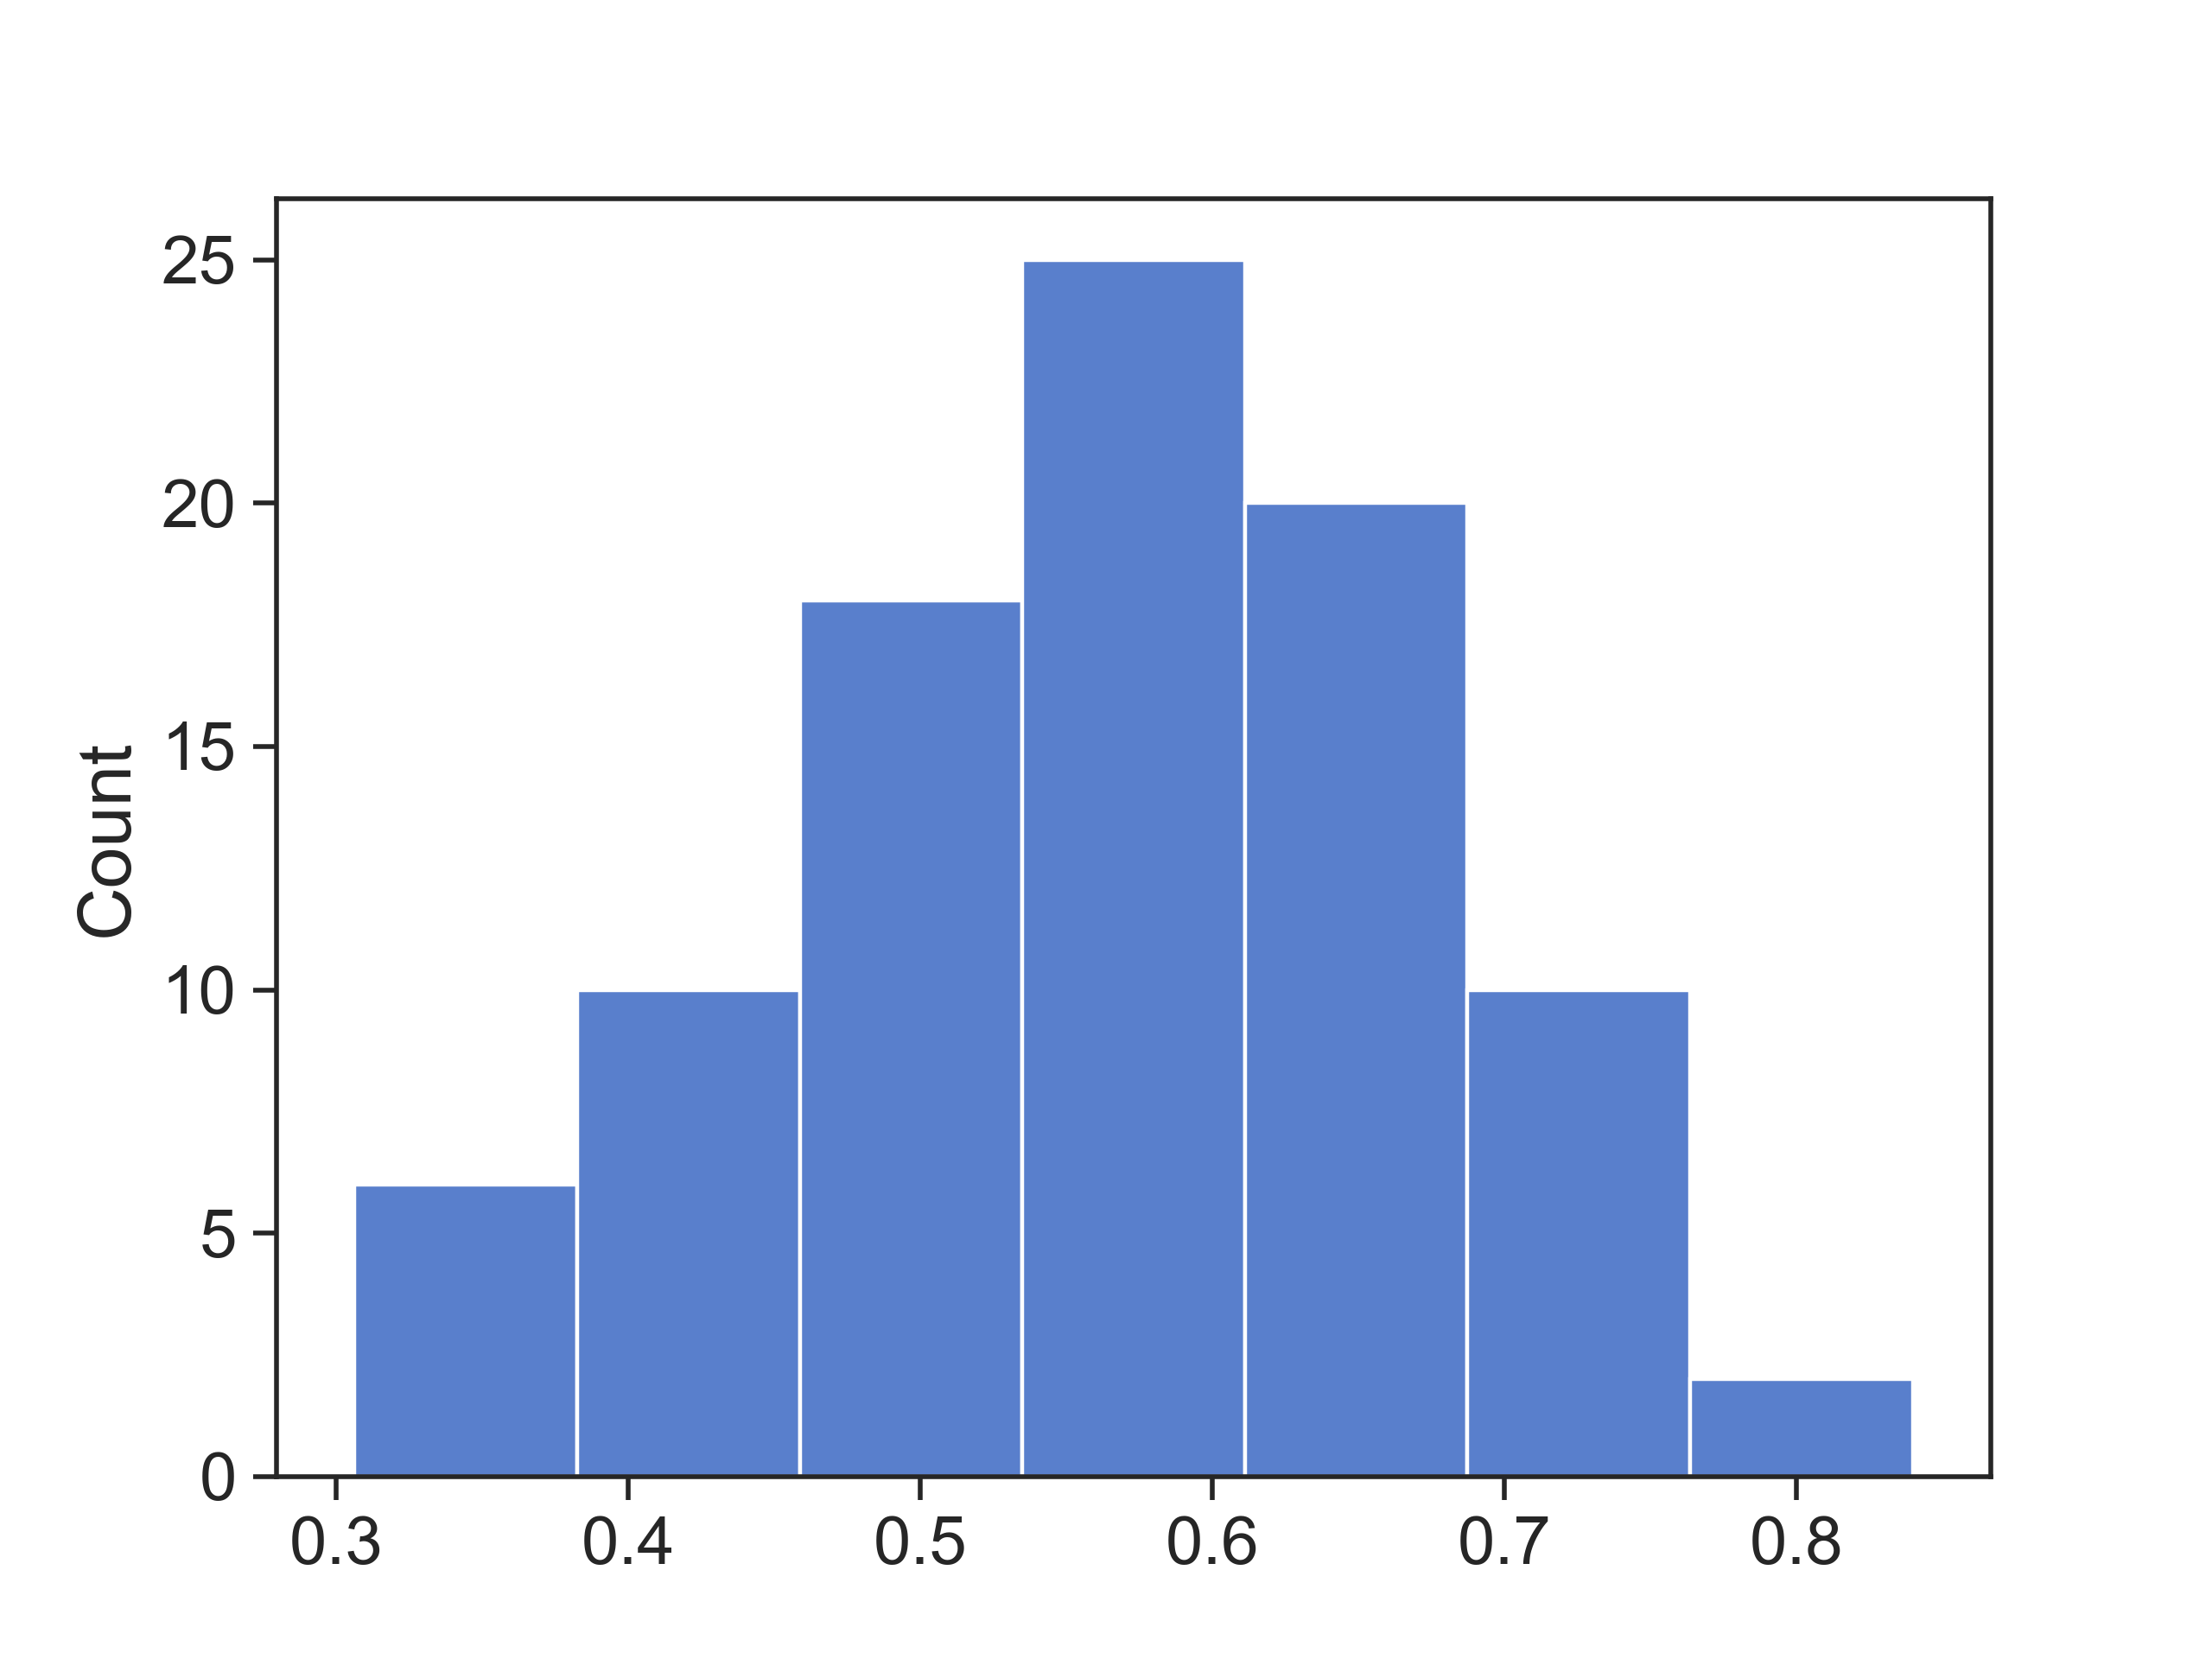
\includegraphics[width=\textwidth]{figures/cons_40.png}
            \caption{QM region $+$ ARG 264, ARG 249, GLN 113 and SER 114 constrained.}
            \label{fig:b}
        \end{minipage}
    \end{figure}
\end{frame}
%
\begin{frame}
%\frametitle{Free energies from TPS}
%\begin{figure}
%\includegraphics[scale=0.25]{hist_path/non_reac_path.pdf}
%\end{figure} 
%\pause
    \begin{figure}[ht]
        \begin{minipage}[b]{0.45\linewidth}
            \centering
            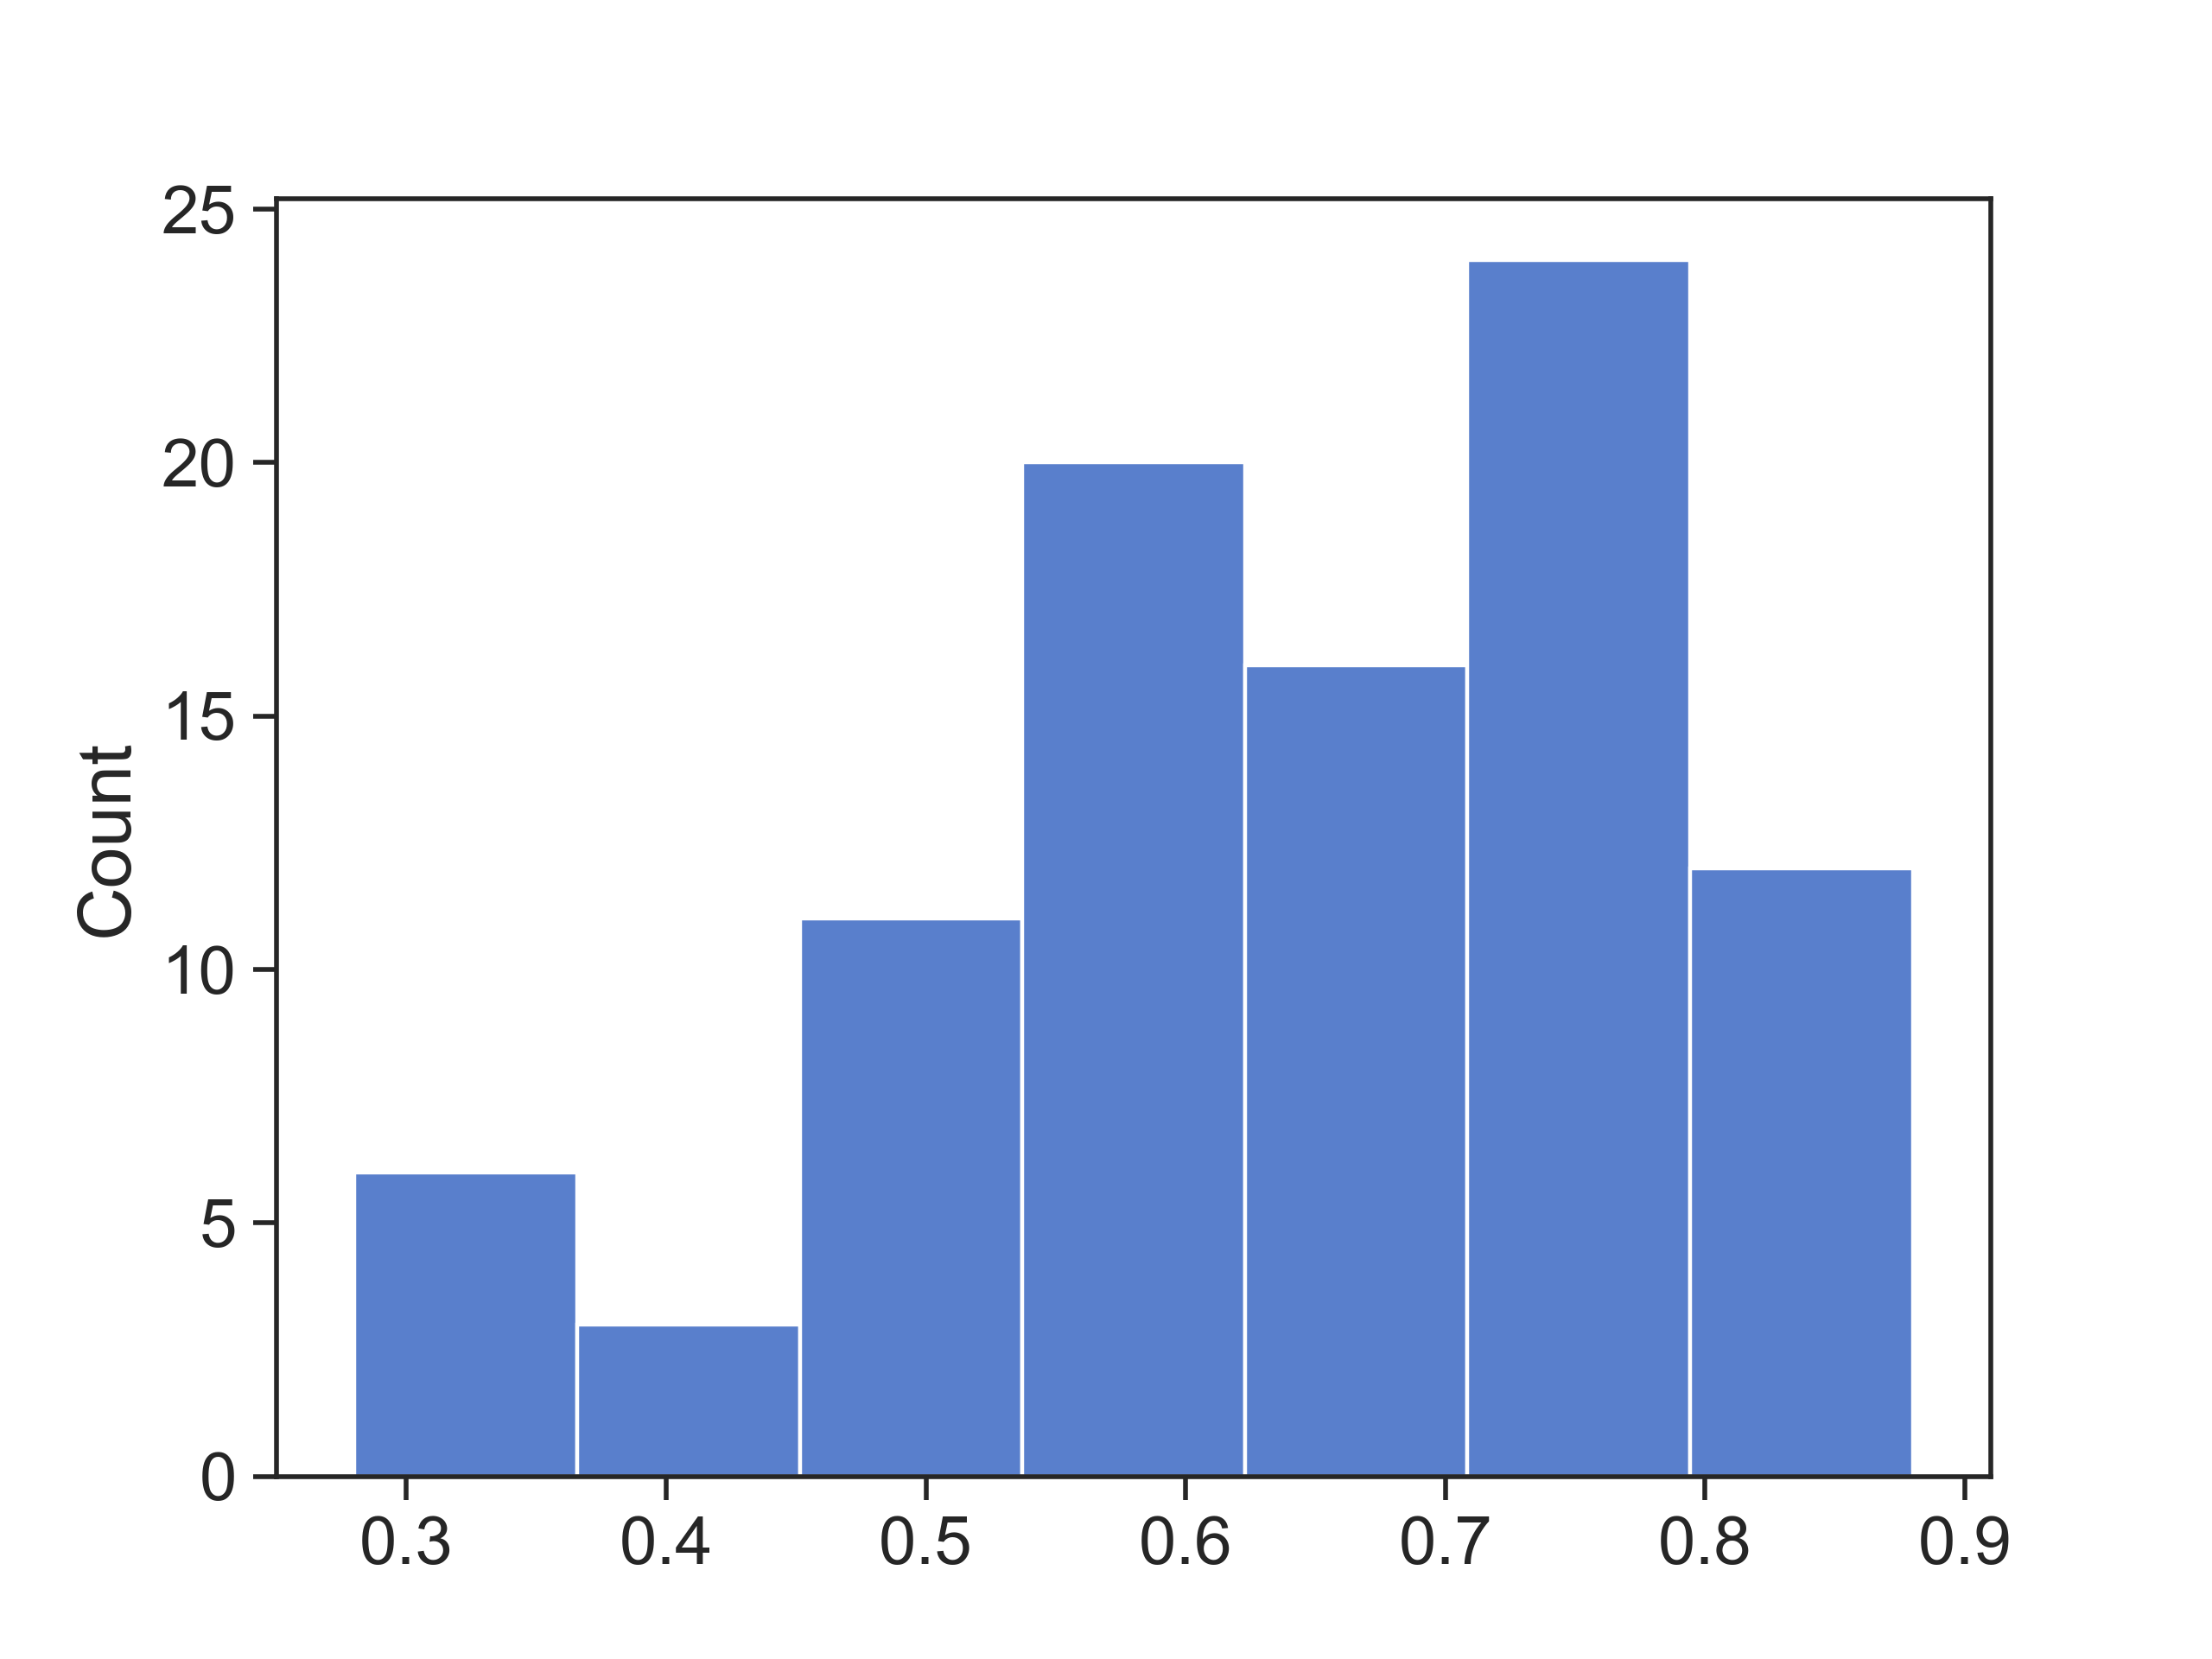
\includegraphics[width=\textwidth]{figures/140.png}
            \caption{QM region constrained.}
            \label{fig:a}
        \end{minipage}
        \hspace{0.5cm}
        \begin{minipage}[b]{0.45\linewidth}
            \centering
            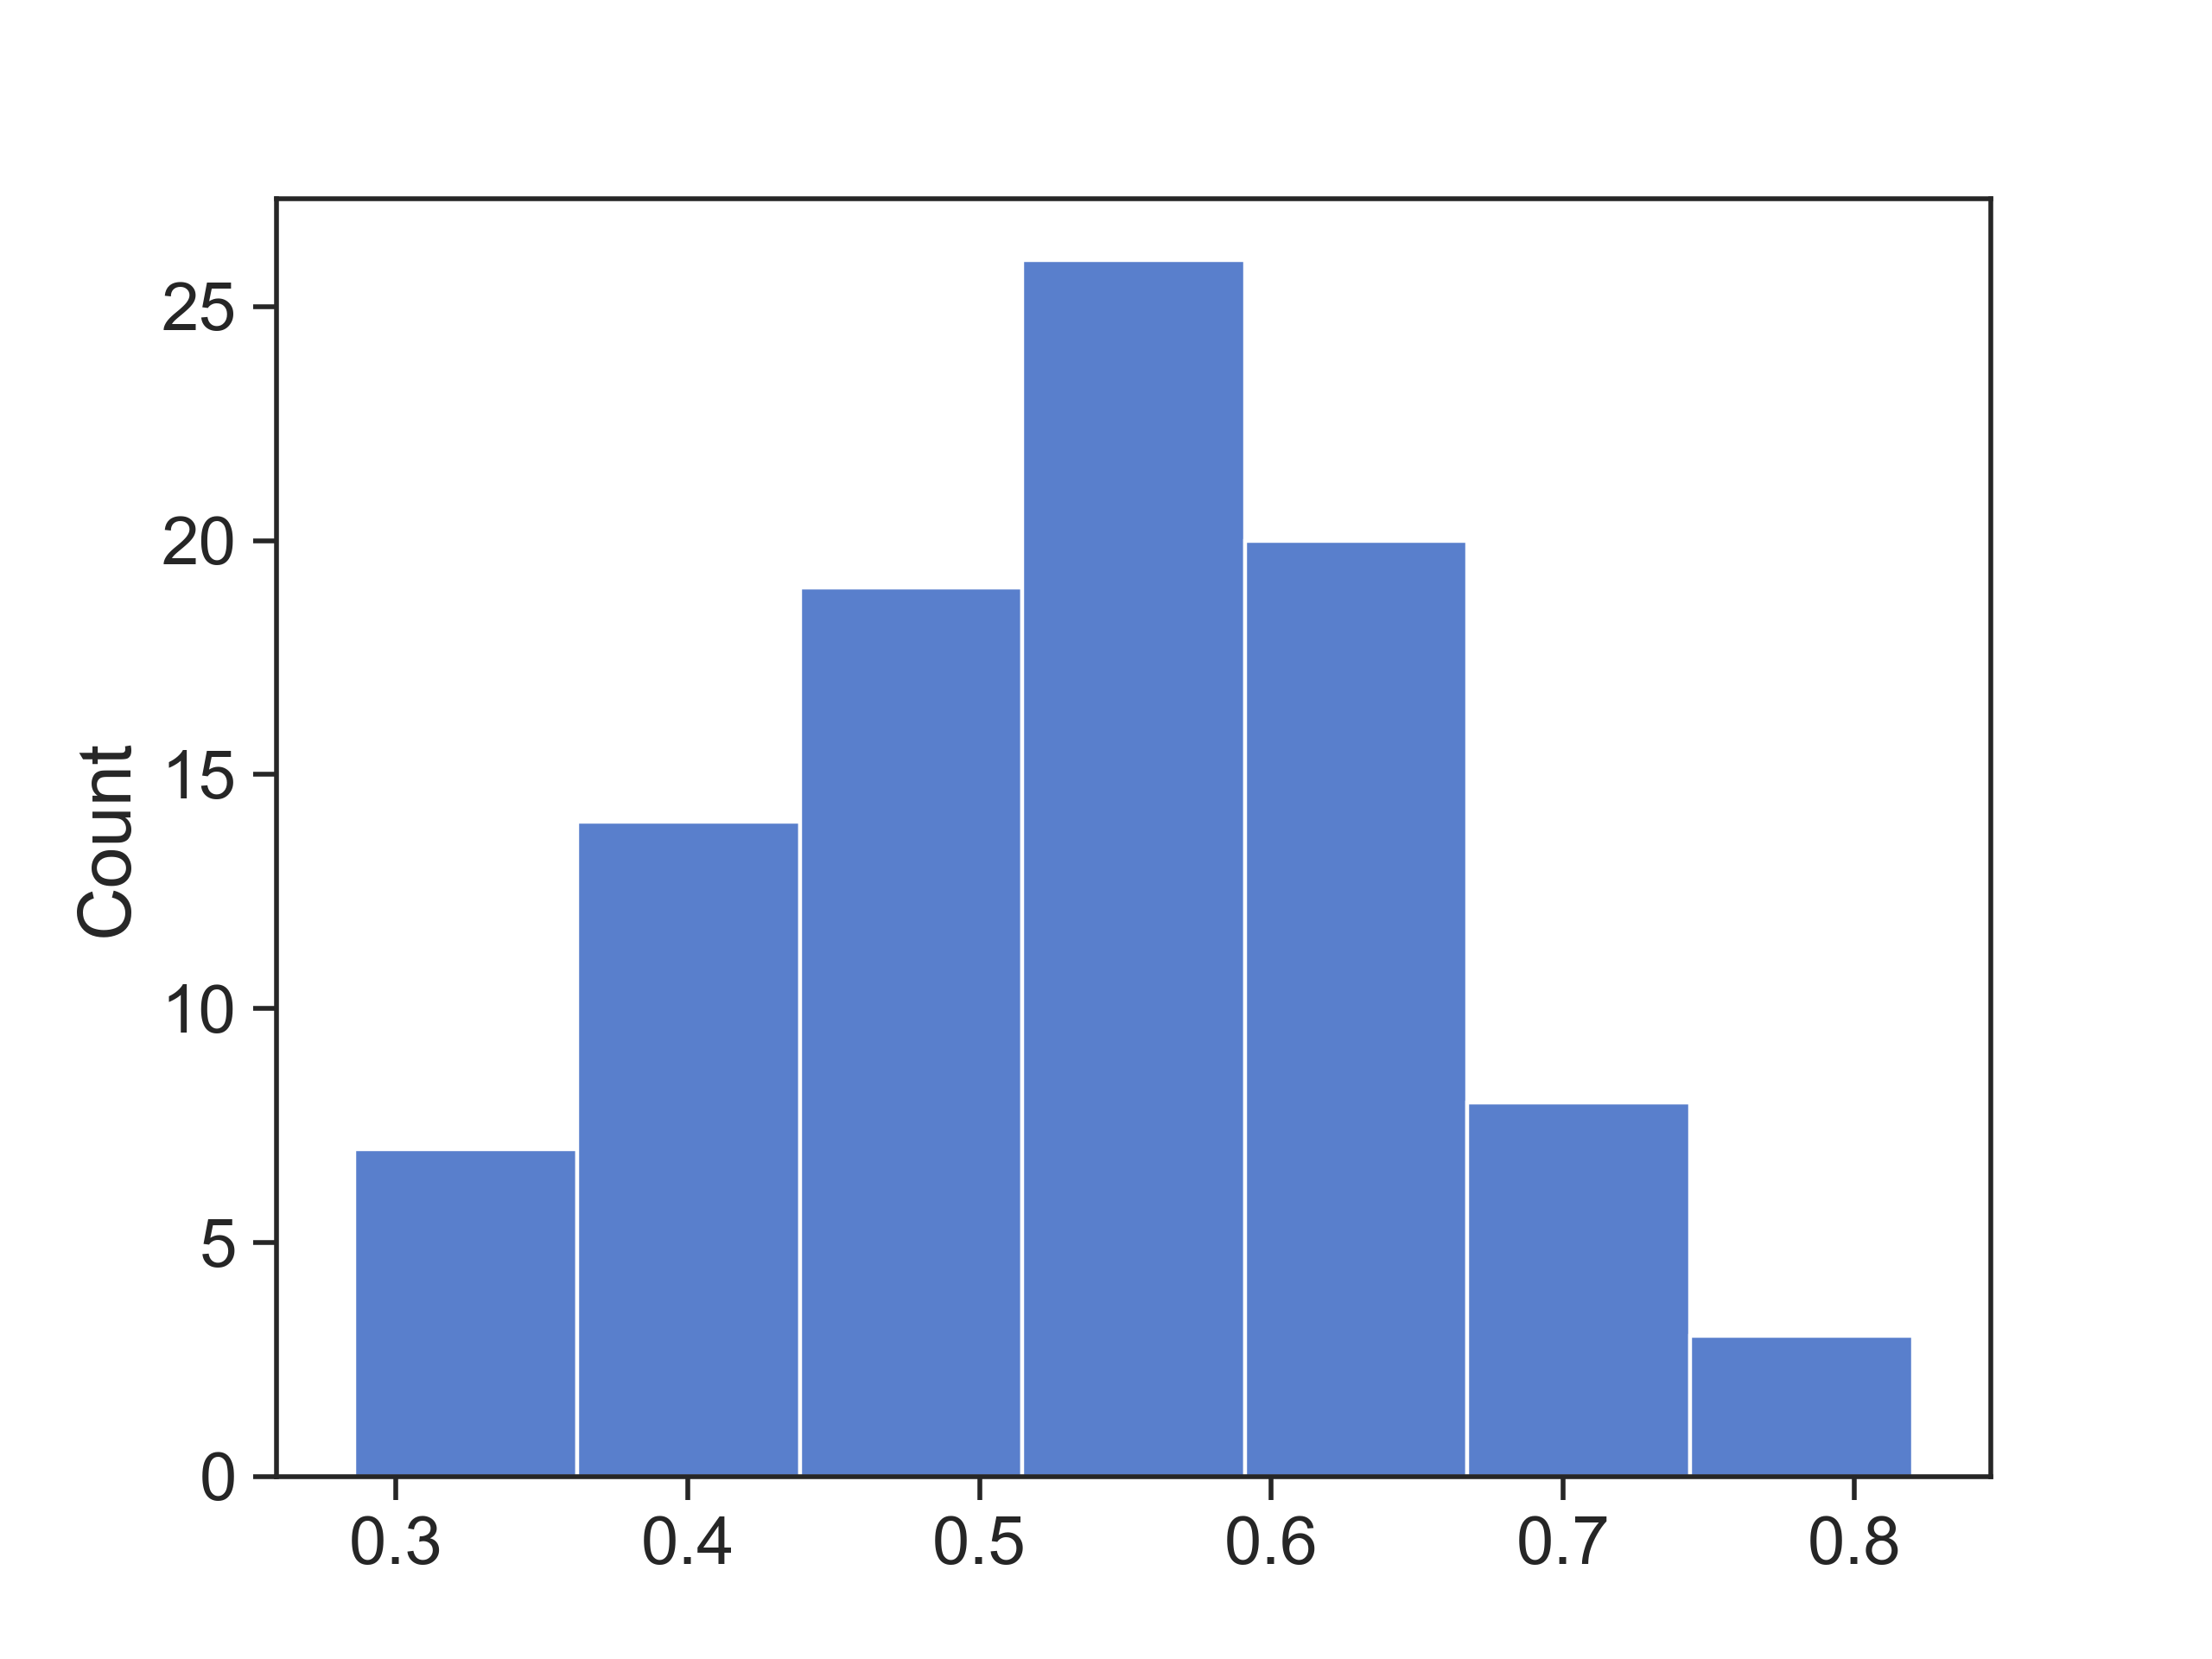
\includegraphics[width=\textwidth]{figures/cons_140.png}
            \caption{QM region $+$ ARG 264, ARG 249, GLN 113 and SER 114 constrained.}
            \label{fig:b}
        \end{minipage}
    \end{figure}
\end{frame}
\begin{frame}
\begin{figure}
\centering
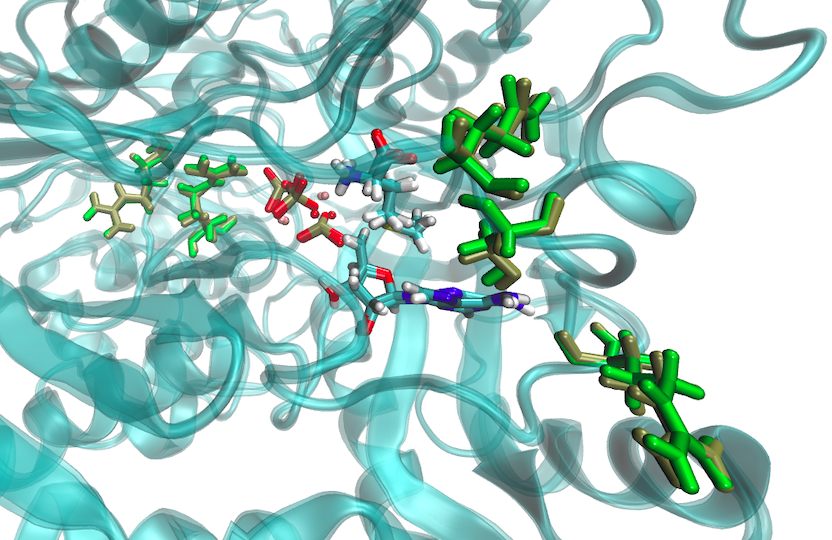
\includegraphics[scale=0.4]{figures/tsdiff.png}
\caption{O-S distances for the TS are $2.416\;$\AA and $2.255\;$\AA. The S-C distances for the TS are $2.127\;$\AA and $2.030\;$\AA}
\end{figure}
\end{frame}

%

%
%
%
%\begin{frame}
%\frametitle{Combining the probabilities in the individual windows}
%Weighted histogram analysis method (WHAM).
%\begin{equation}
%P(\lambda) = \sum^{windows}_j w(\lambda_j)P(\lambda_j) \nonumber 
%\end{equation}
%The weights $w_j$ are chosen to minimize the statistical error of $P(\lambda)$
%\begin{equation}
%\frac{\partial^2\sigma(P(\lambda))}{w(\lambda_j)} = 0 \nonumber 
%\end{equation}
%such that $\sum_jw(\lambda_j)=0$.
%Optimal weights are obtained by solving a set of coupled equations. 
%\end{frame}

\end{document}
